\documentclass{beamer}
%\usepackage[usenames,dvipsnames]{xcolor}

\usepackage{_defsAndPackages675notation}
\usepackage{_defsAndPackages675beamer}

\begin{document}

\title{\alg{Linear Methods for Regression:
Subset selection}}
\subtitle{\classTitle}
%\author{\alg{Darren Homrighausen, PhD}}
%\institute{\classTitle}
\date{}



\begin{frame}
\maketitle
%\titlepage
%\begin{figure}[h!]
%  \centering
%  \includegraphics[width=1in]{.../figures/CSU_logo2.eps}
%\end{figure}
%
\organization
%
\end{frame}

\begin{frame}[fragile]
\frametitle{Summary}
The overall scheme is a three(four?)-fold process
\begin{enumerate}
\item Select a method suited to your task
\item Choose a risk estimation method that has the properties that you desire (e.g. end of previous slides)
\item \textcolor<2>{redmain}{Perform the necessary computations to minimize \textcolor{bluemain}{2.} constrained
to be in the family of procedures in \textcolor{bluemain}{1.}}
\item Show theoretically that your procedure has desirable properties
\end{enumerate}
\end{frame}



\transitionSlide{Brief optimization and convexity detour}

\begin{frame}[fragile]
\frametitle{Optimization}
An optimization problem (program) can be generally formulated as
\begin{align}
\textrm{minimize } & F(x) \\
\label{eq:constraint1}
\textrm{subject to } 
& f_j(x) \leq 0 \textrm{ for }  j = 1, \ldots, m \\
\label{eq:constraint2}
& h_k(x) = 0 \textrm{ for }  k = 1, \ldots, q
\end{align}
Here
\begin{itemize}
\item[] $x = (x_1, \ldots, x_n)^{\top}$ are the \alg{parameters}
\item[] $F:\R^n \rightarrow \R$ is the \alg{objective function}
\item[] $f_j,h_k:\R^n \rightarrow \R$ are \alg{constraint functions}
\end{itemize}

\vsp
The \alg{optimal solution} $x^*$ is such that $F(x^*) \leq F(x)$ for any $x^*,x$ that satisfies equations (\ref{eq:constraint1}) and (\ref{eq:constraint2}).
\end{frame}

\begin{frame}[fragile]
\frametitle{Convexity}
The main dichotomy of optimization programs is  \alg{convex} vs. \alg{nonconvex}
\vsp

Generally speaking, a \alg{convex} program is one in which the objective and contraint functions are all convex,
that is $\forall t \in [0,1], \forall x \in D = \left(\bigcap_{j =1}^m \textrm{dom } f_i \right) 
\cap \left(\bigcap_{k=1}^q \textrm{dom } h_k\right) \cap \left(\textrm{dom F}\right)$, and 
$\forall f \in \{ f_1,\ldots, f_m, h_1,\ldots,h_q, F\}$
\[
f(tx + (1-t)x') \leq tf(x) + (1-t)f(x')
\]
This can be thought of (for smooth enough $f$)
\[
f(x') \geq f(x) + (\nabla f|_x)^{\top} (x' - x) 
\]

\emphasis{8cm}{Intuition:}{This means that the function values at a point $x'$ are \alo{above}
the supporting hyperplane given by the tangent space at \alo{any} point $x$}

\end{frame}

\begin{frame}[fragile]
\frametitle{Convexity example}

\begin{figure}[!h]
\includegraphics[width=3.25in,trim=0 40 0 0,clip]{../figures/3dSquaredErrorOnly.pdf}
\caption*{$\norm{Y - \X\beta}_2^2$ for $p = 2$}
\end{figure}

\end{frame}



\begin{frame}[fragile]
\frametitle{Convexity}
Methods  for convex optimization programs are (roughly) always \alo{global} and \alo{fast}

\vsp
For general nonconvex problems, we have to give up one of these:
\begin{itemize}
\item Local optimization methods that are fast, but need not find global solution

\script{So called \alg{greedy} approximations}
\item Global optimization methods that find global solutions, but
are not always fast (indeed, are often slow)

\script{Usually exhaustive search type approaches}
\end{itemize}
\end{frame}


\transitionSlide{Model selection}
\begin{frame}
\begin{center}
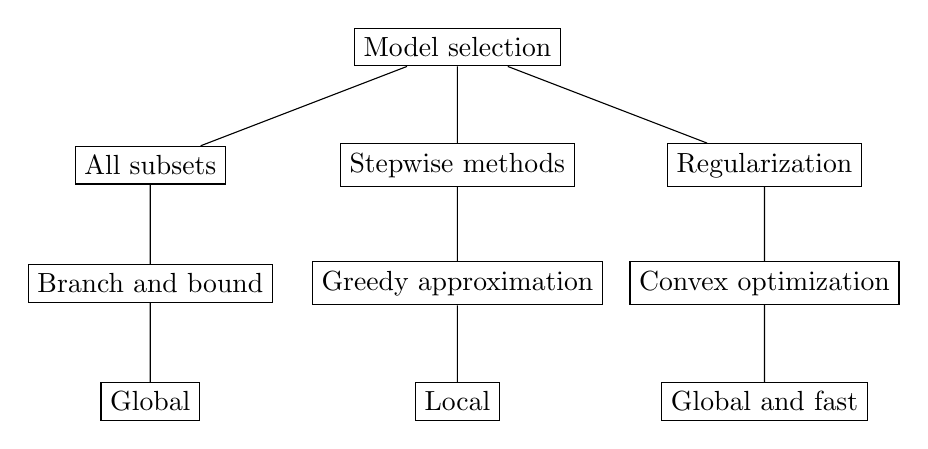
\begin{tikzpicture}
    \tikzstyle{every node}=[rectangle,draw]
    \tikzstyle{level 1}=[sibling distance=39mm] 
    \tikzstyle{level 2}=[sibling distance=23mm]     
    \node {\smallCapGreen{Model selection}}
            child { node {\alr{All subsets}}
            	child { node {\alr{Branch and bound}}
			child { node {\alo{Global}}}
		} 
            }
            child { node {\alr{Stepwise methods}} 
            	child { node {\alr{Greedy approximation}}
			child { node {\alo{Local}}}
		} 
            }
        	   child { node {\alb{Regularization}}           
            	child { node {\alb{Convex optimization}}
			child { node {\alb{Global and fast}}}
		} 
            }
         ;
\end{tikzpicture}
\end{center}
\vsp

Some comments:
\begin{itemize}
\item[] \alr{Non convex programs}
\item[] \alb{Can be seen as a convex relaxation of the nonconvex program giving all subsets}\footnote{We'll
return to this shortly}
\end{itemize}
\end{frame}


\begin{frame}[fragile]
\frametitle{All Subsets Regression}
First, identify all considered covariates and transformation and put 
them in the feature matrix $\X \in \R^{n \times p}$

\vsp
\smallCapGreen{Best subset selection algorithm:}  For $k = 1, \ldots, p$
\begin{enumerate}
\item Find $\train$ for the ${p \choose k}$ models of size $k$
\item Save the model that minimizes $\train$
\end{enumerate}
\vsp

Now, report the model that minimizes one of the risk estimates from the previous
slide over these $p$ models

\end{frame}


\begin{frame}[fragile]
\frametitle{All Subsets Regression in {\tt R}} 
We can find with the function \alr{regsubsets} in the package \alr{leaps}

\script{See code on website}
\vsp
The syntax and associated objects look like:
\begin{blockcode}
allsubsets.out = regsubsets(Y~.,data=X,nvmax=pmax)
> summary(allsubsets.out)
[1] "which"  "req"  "rss"  "adjr2"  "cp"  "bic  "outmat"  "obj"
\end{blockcode}
\begin{itemize}
\item The \alr{nvmax = pmax} controls the max size of models considered.  The default is 8 and that is usually far too small.
\item Now, we can pick among the \alr{pmax}  models that minimize $\hat{R}$ for a given model size using BIC or Cp
\end{itemize}
\vsp

This can be done in some cases, though there is a problem
\end{frame}



\begin{frame}[fragile]
\frametitle{All Subsets Regression: A Big Problem  (Literally)}
If there are $p$  predictors  then there are \alo{$2^p $ possible models} 

\script{Without considering interactions or transformations}

\vsp
In general, this is a nonconvex problem 
\vsp

If $p = 40$
(which is considered a small problem these days), then the number of possible models is
\[
2^{40} \approx 1,099,512,000,000 \Rightarrow \textrm{More than 1 trillion!}
\]

\vsp
If $p = 265$, then the number of possible models is more than the \alo{number of atoms
in the universe}\footnote{It is estimated there are $10^{80}$ atoms in the universe.}

\vsp
We must sift through the models in a computationally feasible way
\end{frame}

\begin{frame}[fragile]
\frametitle{All Subsets Regression}
The \alr{leaps} package in \alr{R} uses a technique known as
\alg{branch and bound}

\script{The statistical implementation is based on the paper Furnival and Wilson (1974)}
\vsp

It is a widely used tool for solving large scale NP-hard combinatorial optimization problems.

\vsp
Note, however, that though it can speed up the optimization immensely, it cannot reduce the complexity
of the problem 

\script{Still exponential}
\end{frame}

\begin{frame}[fragile]
\frametitle{Branch and bound}
Let $M = M_1\cup \ldots \cup M_K$ be the set of all possible solutions and a partition comprised of \alg{branches}, respectively.  

\script{Statistically, we think of $M$ as the set of all possible models.}


\vsp
Suppose for objective function $F$ we want to find
\[
F_* :=  \max_{m \in M} F(m)
\]

\vsp
For each $M_k$, define
\[
F_k := \max_{m \in M_k} F(m) 
\]
and let $\underline{F}_k, \overline{F}_k $ be a \alg{bracket} such that
\[
 \underline{F}_k \leq F_k \leq \overline{F}_k 
\]
\script{Note that $F_k$ is in general not explicitly constructed}
\vsp

Then
\[
\max_k \underline{F}_k := \underline{F} \leq F_* %\leq \overline{F} := \max_k \overline{F}_k
\]
\end{frame}

\begin{frame}[fragile]
\frametitle{Branch and bound}
The main realization is that the \alg{branch} $M_k$ does not need to be explored if
either of the following occur
\begin{itemize}
\item[i.] \smallCapGreen{Bound}
\[
\overline{F}_k \leq \underline{F}
\]
\item[ii.] \smallCapGreen{Optimality}
\[
\max_{m \in M_k} F(m) \textrm{ has been found}
\]
\end{itemize}
\vfill

\end{frame}

\begin{frame}[fragile]
\frametitle{Branch and bound}
The two main questions remain:
\begin{enumerate}
\item How to choose the partition(s)?
\item How to form the \alo{bracket}?

\script{Note that to be helpful, the bracket must be easy to compute}
\end{enumerate}

\vvsp
These are very case specific.  Let's return to model selection
\end{frame}

\begin{frame}[fragile]
\frametitle{Branch and bound for model selection}
Let's suppose we set\footnote{Note: we are trying to minimize $F$, not maximize}
\[
F(m) = n \log(\train(\hat\beta_m)) + 2|m| 
\]

For a set of models $M_k$, let
\begin{itemize}
\item[] $m_{k,inf}$ be the largest model contained\footnote{This does not have to be in $M_k$}
 in every model in $M_k$
\item[] $m_{k,sup}$ be a smallest model that contains every model in $M_k$
\end{itemize}

\end{frame}

\begin{frame}[fragile]
\frametitle{Branch and bound for model selection}
\textbf{Example:} Let $x_1, \ldots, x_5$ be covariates

\[
M  = \cup_{k=1}^3 M_k,
\]
where
\begin{align*}
M_1 
& = \{\{x_1,x_3\}, \{x_2\} \}, \\
M_2 
& = \{\{x_2,x_3,x_4\}, \{x_3,x_4\} \}, \\
 M_3 
& = \{\{x_3,x_5\}, \{x_3\} \}, 
\end{align*}
\pause

\begin{itemize}
\item[] $m_{2,inf} = \{x_3,x_4\}$
\item[] $m_{2,sup} = \{x_2,x_3,x_4\}$
\end{itemize}


\end{frame}

\begin{frame}[fragile]
\frametitle{Branch and bound for model selection}
\smallCapGreen{Reminder:}

For the $M_k$, let
\begin{itemize}
\item[] $m_{k,inf}$ be the largest model contained
 in every model in $M_k$
\item[] $m_{k,sup}$ be a smallest model that contains every model in $M_k$
\end{itemize}
\vvsp


Then:

\vsp
 $\forall m \in M_k$
\begin{itemize}
\item[] $F(m) \geq n \log(\train(\hat\beta_{m_{k,\sup}})) + 2|m_{k,\inf}| = L_k$  
\item[] $F(m) \leq n \log(\train(\hat\beta_{m_{k,\inf}})) + 2|m_{k,\sup}|  = U_k$ 

\script{We don't actually need $U_k$, though}
\end{itemize}

\end{frame}

\begin{frame}[fragile]
\frametitle{Branch and bound for model selection: An algorithm}
\begin{enumerate}
\item Define a global variable $b = F(m)$ for any $m \in M$

\script{As an aside, every time $F(m)$ is computed, update $b$ if $F(m) < b$} 
\item Partition $M = \{M_1,\ldots,M_K\}$
\item For each $k$, if $L_k > b$, eliminate the branch $M_k$
\item Gather each remaining $M_k$ and set union equal to $M$
\item Else, recurse and return to \textcolor{bluemain}{2.}
\end{enumerate}

\end{frame}

\transitionSlide{Greedy approximations}

\begin{frame}[fragile]
\frametitle{Forward stepwise selection}
In the likely event that $2^p$ is too large to be searched over exhaustively, a common \alg{greedy}
approximation is the following

\vsp
Let $\hat{R}$ be any risk estimate
\begin{enumerate}
\item Find $\hat{R}(\emptyset)$: That is, the intercept only model
\item Search over all $p$ single feature models, computing $\hat{R}$ for each one.  Say including $x_j$
minimizes $\hat{R}$ with a value $\hat{R}(x_j)$.  If $\hat{R}(x_j) < \hat{R}(\emptyset)$, add $x_j$
to the model and continue.  Otherwise terminate
\item Now search over all $p-1$ models that contain $x_j$ and find the $x_{j'}$ that minimizes $\hat{R}$.  
If $\hat{R}(x_j,x_{j'}) < \hat{R}(x_j)$, add $x_{j'}$
to the model and continue.  Otherwise terminate
\item $\cdots$
\end{enumerate}
\end{frame}

\begin{frame}[fragile]
\frametitle{Forward stepwise selection}
\begin{blockcode}
regsubsets(Y~.,data=X,nvmax=pmax,method='forward')
\end{blockcode}

\smallCapGreen{Pros:} 
\begin{itemize}
\item This approach can be used effectively in either the \alb{Big Data} or \alb{High Dimensional} regimes
\item It tends to produce sensible answers that are not too different from all-subsets
\end{itemize}
\vsp

\smallCapGreen{Cons:} 
\begin{itemize}
\item Can get trapped in a poor local minimum
\end{itemize}
\end{frame}

\begin{frame}[fragile]
\frametitle{General stepwise selection}
This algorithm can can adapted to..
\vsp

\begin{itemize}
\item start with the full model and stepwise remove covariates.  This is known as \alg{backward stepwise selection}
\begin{blockcode}
regsubsets(Y~.,data=X,nvmax=pmax,method='backward')
\end{blockcode}
\script{useful if the full model isn't too large and a superset of the important covariates is desired}
\item consider both adding and removing covariates at each step.  This is known as \alg{stepwise selection}
\begin{blockcode}
regsubsets(Y~.,data=X,nvmax=pmax,method='seqrep')
\end{blockcode}

\end{itemize}
\end{frame}

\begin{frame}[fragile]
\frametitle{Important comments}
After using any of these model selection approaches, we produce estimates $\hat\beta$ and predictions 
$\hat{Y} =\hat\beta^{\top} X_{\textrm{select}}$
where $X_{\textrm{select}}$ includes only the selected features

\vsp
This can be interpreted as these covariates are most important for predicting $Y$ from the features included in $X \in \R^p$

\script{The usual caveats apply: linearity (correlation), there are surely some important coefficients left out/unimportant ones included}

\vsp
If we run \alr{out = lm(Y$\sim \X_{\textrm{select}}$)}, then \alr{summary(out)} will produce the usual significance tests: \alo{these are not valid 
after model selection}


\end{frame}

\begin{frame}[fragile]
\frametitle{Important comments}
\begin{itemize}
\item If we want to be sure to include all the important covariates, then we can use AIC/Cp + backward stepwise selection
\item If we want to be sure to only include  important covariates, then we can use BIC + forward stepwise selection
\item If we want to do predictions, use AIC/Cp, but it isn't clear what method is the best
\end{itemize}
\script{See website for example code for doing model selection in \alr{R}}
\end{frame}

\end{document}
